\documentclass[tikz]{standalone}
\usepackage{tikz}
\usetikzlibrary{angles,quotes}
\begin{document}
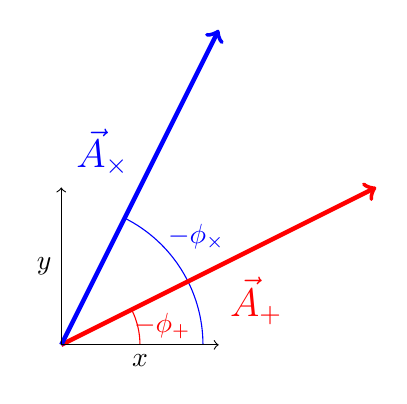
\begin{tikzpicture}%[> = stealth]
\coordinate (o) at (0,0);
\coordinate (c) at (2,4);
\coordinate (p) at (4,2);

\coordinate (x) at (2,0);
\coordinate (y) at (0,2);

%\draw[gray,step=1cm] (0,0) grid +(9cm,6cm);
\draw[blue] pic[draw,angle radius=1.8cm,"$-\phi_\times$" shift={(8mm,8mm)}] {angle=x--o--c};
\draw[red] pic[draw,angle radius=1cm,"$-\phi_+$" shift={(7mm,1mm)}] {angle=x--o--p};

\draw[ultra thick,red, ->]  (o) -- node[below right] {\Large $\vec{A}_+$} (p);
\draw[ultra thick,blue,->]  (o) -- node[above left] {\Large $\vec{A}_\times$} (c);

\draw[thin,black, ->]  (o) -- node[below] {$x$} (x);
\draw[thin,black,->]   (o) -- node[left] {$y$} (y);
\end{tikzpicture}
\end{document}
